\documentclass[11pt,reqno,oneside]{article}
% \documentclass[12pt, final]{siamonline171218}
% \usepackage[pdfborder={0 0 0.5 [3 2]}]{hyperref}%
\usepackage[left=1in,right=1in,top=1in,bottom=1in]{geometry}%
\usepackage{amsmath}
\usepackage{amssymb}
\usepackage{amsthm}
\usepackage{graphicx}
\usepackage{enumerate}
\usepackage{float}
\usepackage{bm}
\usepackage[stable]{footmisc}

\usepackage{packages}
\usepackage{wrapfig}
\usepackage{subfigure}
\usepackage[font=footnotesize]{caption}

\newtheorem{theorem}{Theorem}
\newtheorem{lemma}[theorem]{Lemma}
\newtheorem{corollary}{Corollary}

\theoremstyle{definition}
\newtheorem{definition}[theorem]{Definition}

\theoremstyle{remark}
\newtheorem{remark}[theorem]{Remark}

\def\noi{\noindent}
\def\T{{\mathbb T}}
\def\R{{\mathbb R}}
\def\N{{\mathbb N}}
\def\Z{{\mathbb Z}}
\def\C{{\mathbb C}}
\def\Q{\mathbb{Q}}

\newcommand{\vK}{\bm{\mathit{K}}}
\newcommand{\calP}{\mathcal{P}}
\newcommand{\calA}{\mathcal{A}}

\setlength{\parindent}{0em}
\setlength{\parskip}{1em}
\renewcommand{\baselinestretch}{1.1}

\title{Research Statement}
\date{\vspace{-12ex}}

\begin{document}

\thispagestyle{empty}

% \maketitle

\subsection*{Scientific Summary}

My main research focus is on understanding patterns and coherent structures arising in the natural sciences and engineering. Mathematically, these are described by nonlinear evolution equations, which take the form of partial differential equations (PDEs) or systems of ordinary differential equations (ODEs). Most of the systems I study are nonlinear wave equations, which describe the time evolution of a function representing a wave profile. Coherent structures are spatial patterns which maintain their shape as the system evolves in time. Examples of coherent structures include solitary waves, which are localized disturbances that propagate at a constant velocity, and breathers, which are disturbances that are localized in space but oscillate in time. 
Solitary waves have been a topic of interest since the 19th century, when John Scott Russell observed a single, large surface wave on the Edinburgh-Glasgow Union Canal in Scotland; this phenomenon was explained mathematically 60 years later by the Korteweg–de Vries (KdV) equation.
Although solitary waves were originally discovered as a water wave phenomenon, they have applications in many fields, including fiber optics, plasma physics, quantum mechanics, molecular biology, and neuroscience. More generally, many nonlinear, dispersive PDEs exhibit solitary wave solutions. My research falls into two broad categories. First, I study the existence and spectral stability of complex structures in Hamiltonian systems; these systems are characterized by a conserved quantity, such as energy, that remains constant in time. These patterns are constructed using simpler objects, such as solitary waves, as building blocks. 
Second, I study localized patterns in lattices of optical fibers. These mathematical models are inspired by recent advances in experimental optics. Finally, some very recent work explores bifurcation structures in neural network models in the presence of symmetries in the connectivity matrix describing the network.

\subsection*{Research Program}

The bulk of my published research concerns coherent structures in Hamiltonian systems. At a high level, I start with a simple coherent structure, such as a solitary wave, and use it as a building block to construct more elaborate structures. I then study the stability of these more complicated structures in terms of their underlying geometry, together with properties of the simpler structure. The prototypical nonlinear wave equation has a primary solitary wave solution, also known as a primary pulse solution, which looks like a single localized ``bump''. In many systems, multi-pulse solutions also exist; these are ``multi-bump'' solitary waves which resemble multiple, well-separated copies of the primary pulse. The entire multi-pulse travels as a unit, and maintains its shape unless perturbed. In addition to having applications in nonlinear optics and neuroscience, multi-pulses are interesting mathematically. In my research, I explore the existence and stability of these multi-pulse structures. A crucial step in this process is determining the spectrum of the linearization of the underlying system about a multi-pulse. When a multi-pulse is perturbed, interactions between the individual pulses in the structure are revealed, which are a consequence of the inherent nonlinearity of the system. The dynamics of these interactions are determined by the eigenvalues of the linearized system and their corresponding eigenfunctions.

\begin{figure}
    \centering
    \begin{tabular}{cc}
        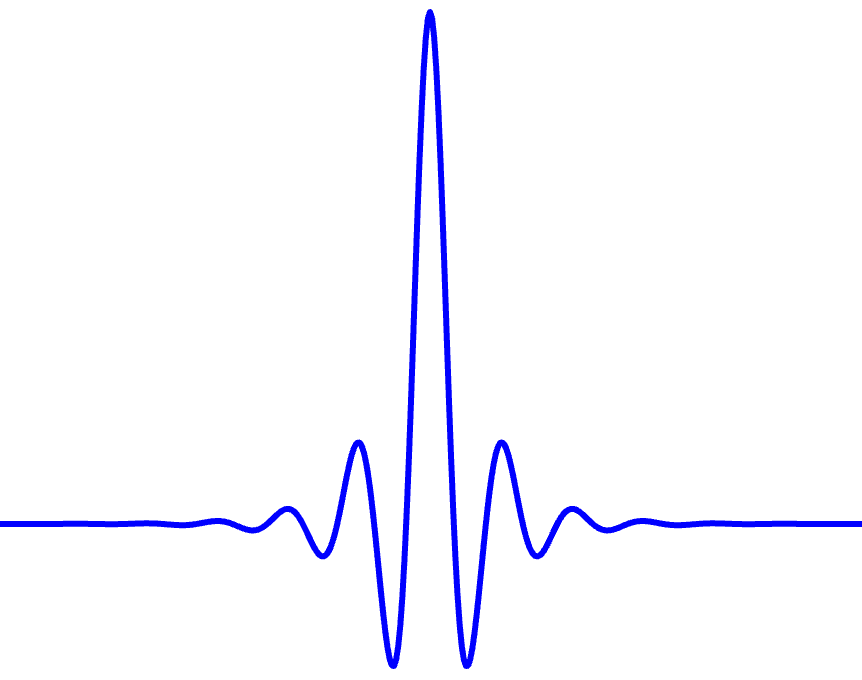
\includegraphics[width=4.5cm]{images/linchen1.png} &
        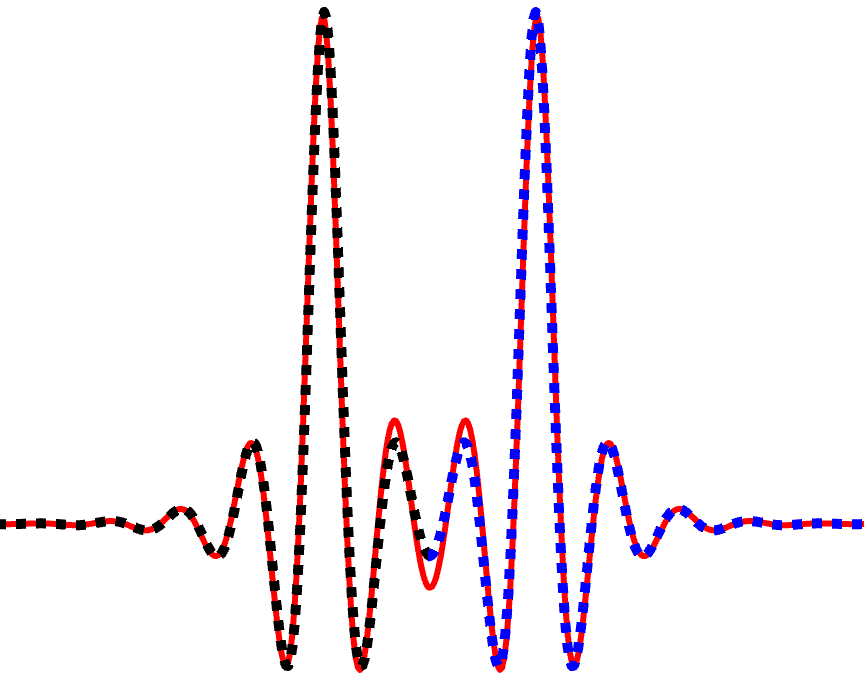
\includegraphics[width=4.5cm]{images/linchen2.png} 
    \end{tabular}
    \caption{Cartoon illustrating construction of a double pulse solution using Lin's method. Left panel shows primary pulse solution. Right panel shows two copies of the primary pulse solution (black and blue dotted lines) placed end-to-end. Double pulse solution (red solid line) is close, but not equal, to this.}
    \label{fig:linsmethod}
\end{figure}

My mathematical approach to this problem comes from spatial dynamics. From this viewpoint, a solitary wave is a homoclinic orbit evolving in the spatial variable $x$, and multi-pulses are multi-loop homoclinic orbits. Multi-pulses can be constructed using Lin's method, a version of the Lyapunov-Schmidt reduction, which can be used to find solutions that are close to a homoclinic orbit. Heuristically, this process involves ``gluing together'' multiple copies of the primary pulse solution end-to-end using small remainder functions (\cref{fig:linsmethod}). The existence of multi-pulse solutions is constrained by the geometry of the primary pulse and the underlying system. In \cref{fig:linsmethod}, for example, multi-pulses can only be constructed  when the tail oscillations of the individual pulses overlap in-phase. In general, each pulse that is added to a multi-pulse structure is associated with one or more eigenvalues in the spectrum, which I call interaction eigenvalues, since they result from nonlinear interactions between the tails of neighboring pulses. Since the systems I study are Hamiltonian, all eigenvalues must come in quartets of the form $\pm \alpha \pm \beta i$. Although this additional structure is helpful, it also means that the presence of any eigenvalue with nonzero real part implies that there is an unstable eigenvalue with positive real part. As a consequence, Hamiltonian systems cannot be dissipative, which makes stability analysis more difficult. 

Some specific examples of Hamiltonian equations I study include
\begin{align*}
i \dot{u}_n + d(u_{n+1} - 2 u_n + u_{n-1}) + |u_n|^2 u_n &= 0 &&\text{discrete nonlinear Schr{\"o}dinger equation (DNLS)} \\
u_{tt} + u_{xxxx} + \mathrm{e}^{u-1} - 1 &= 0 &&\text{Chen-McKenna suspension bridge equation} \\
% \partial_t u - \partial_x^5 u + \partial_x^3 u + 2 u \partial_x u &= 0 && \text{fifth-order Korteweg de-Vries equation (KDV5)} 
i u_t + \frac{\beta_4}{24}u_{xxxx} - \frac{\beta_2}{2}u_{xx} + \gamma |u|^2 u &= 0 && \text{fourth-order nonlinear Schr{\"o}dinger equation (NLS4)}
\end{align*}
My main results relate the spectral pattern of the interaction eigenvalues to the underlying geometry of the multi-pulse. In all cases, the spectral pattern is determined by this geometry. 
DNLS is an analogue to the nonlinear Schr{\"o}dinger equation on the integer lattice, and has applications to nonlinear optics and condensed matter physics. 
% The parameter $d$ quantifies the coupling between adjacent lattice nodes. 
For DNLS, I prove that multi-pulses exist as long as neighboring peaks are either in-phase or out-of-phase. The only stable multi-pulses are those for which all consecutive peaks are out-of-phase. The proof uses Lin's method to construct the eigenfunctions associated with the interaction eigenvalues, which reduces the spectral problem to finding the eigenvalues of a matrix. 
The Chen-McKenna suspension bridge equation is a smooth approximation to a model for waves propagating on an infinitely long suspended beam, and is motivated by observations of traveling waves on suspension bridges. For Chen-McKenna, I prove that the stability pattern is determined by the distances between consecutive peaks, which are constrained to be a multiple of a phase parameter. The proof uses the Krein matrix, which is a projection of an eigenvalue problem onto a finite dimensional subspace. NLS4 is a variant of the nonlinear Schr{\"o}dinger equation which motivated by recent experiments, and was introduced to account for the role of small fourth-order dispersion terms in the propagation of intense laser beams in a bulk medium with Kerr nonlinearity. For NLS4, I prove that multi-pulses exist, but are all unstable due to the presence of an eigenvalue with positive real part. Other systems I have studied include multi-loop periodic orbits in the fifth-order KdV equation, and multi-kinks in the discrete sine-Gordon equation. Ongoing research includes multi-breathers in the discrete Klein-Gordon equation.

There has been much recent interest in the field of topological photonics, as experimental physicists and engineers have developed new techniques for controlling light propagation in photonic crystals and optical fibers. One specific application is light transmission through multi-core optical fibers. In particular, optical transmission properties can be tuned by introducing a twist to the fiber bundle. The propagation of light through a twisted optical fiber comprising $N$ waveguides arranged in a circle is described by the coupled mode equations
\begin{align*}
i \frac{d}{dz} c_n &= k \left(e^{-i\phi}c_{n+1} + e^{i\phi}c_{n-1}\right) + |c_n|^2 c_n &&  n = 1, \dots, N,
\end{align*}
where $z$ is the axis of propagation, $k$ is the strength of the nearest-neighbor coupling, and $\phi$ is a parameter representing the twist of the fiber. When the twist parameter $\phi$ and the number of fibers $N$ are related by $\phi = \pi/N$, I prove that there is a stable standing wave solution of the form $c_n(z) = a_n e^{i \omega z}$ which has a ``dark node'' with no optical activity opposite a ``bright node'' of maximum intensity. I also use an asymptotic approach to show that the same phenomenon occurs if the model incorporates a second-order temporal dispersion term. More recent work involves a model of a waveguide consisting of a square lattice of fibers, in which there are periodic variations along the waveguide axis causing the nearest-neighbor coupling to vary periodically in $z$ (\cref{fig:Rechtsman}, left). In particular, for any $z$, a waveguide is coupled to only one of its four neighbors. This configuration gives rise to localized periodic breather solutions, in which the bulk of the optical intensity is confined to a single square in the lattice but ``jumps'' around that square counterclockwise (\cref{fig:Rechtsman}, middle and right). 
\begin{figure}
    \centering
    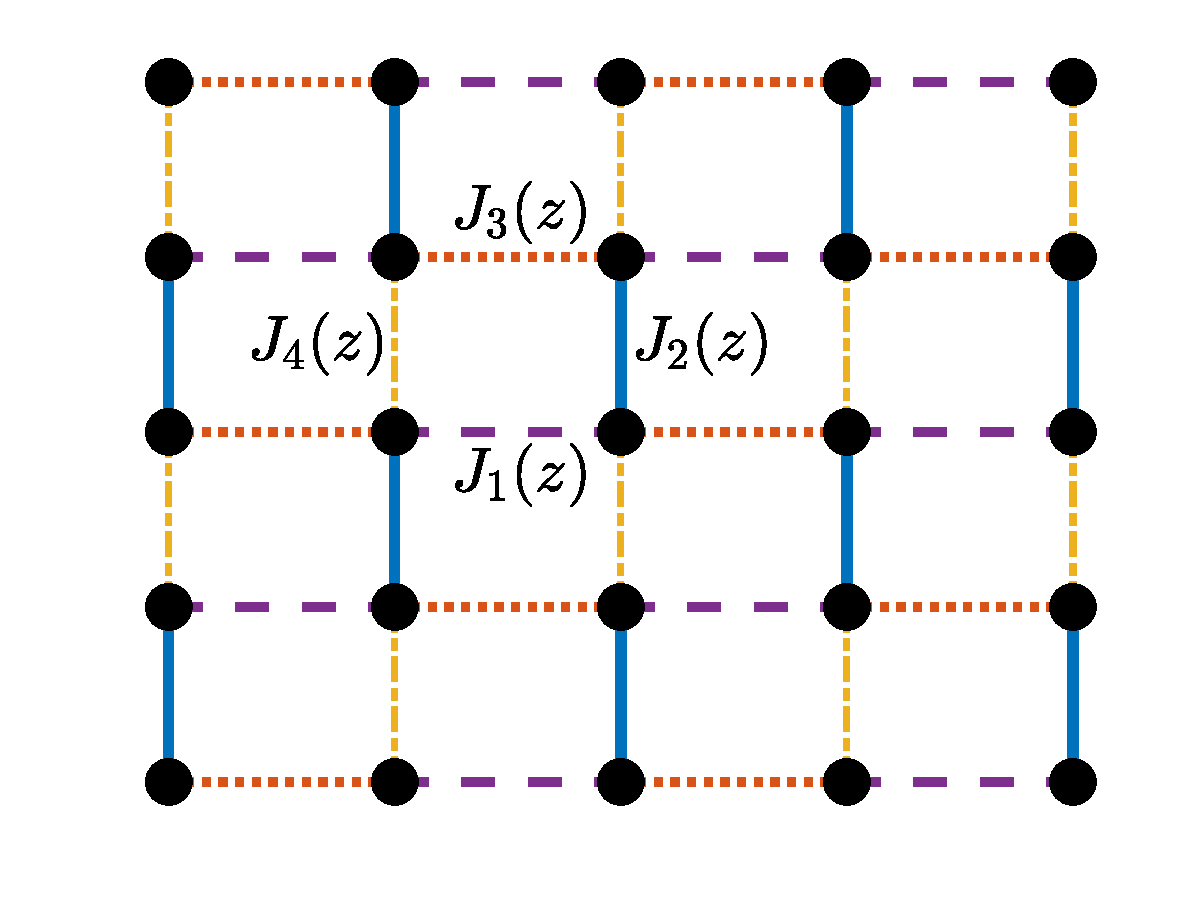
\includegraphics[width=4.5cm]{images/lattice.eps}
    % 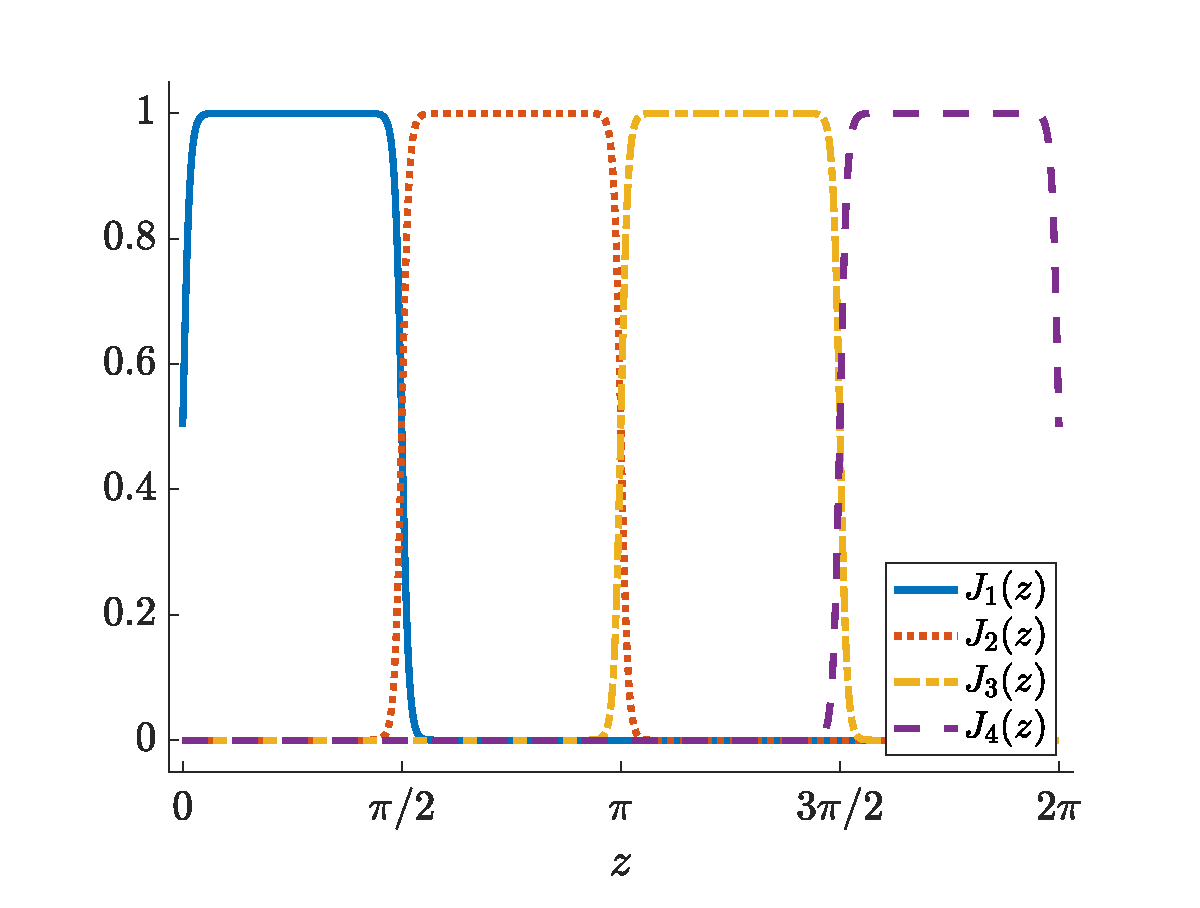
\includegraphics[width=7.8cm]{images/Jplot.eps}
    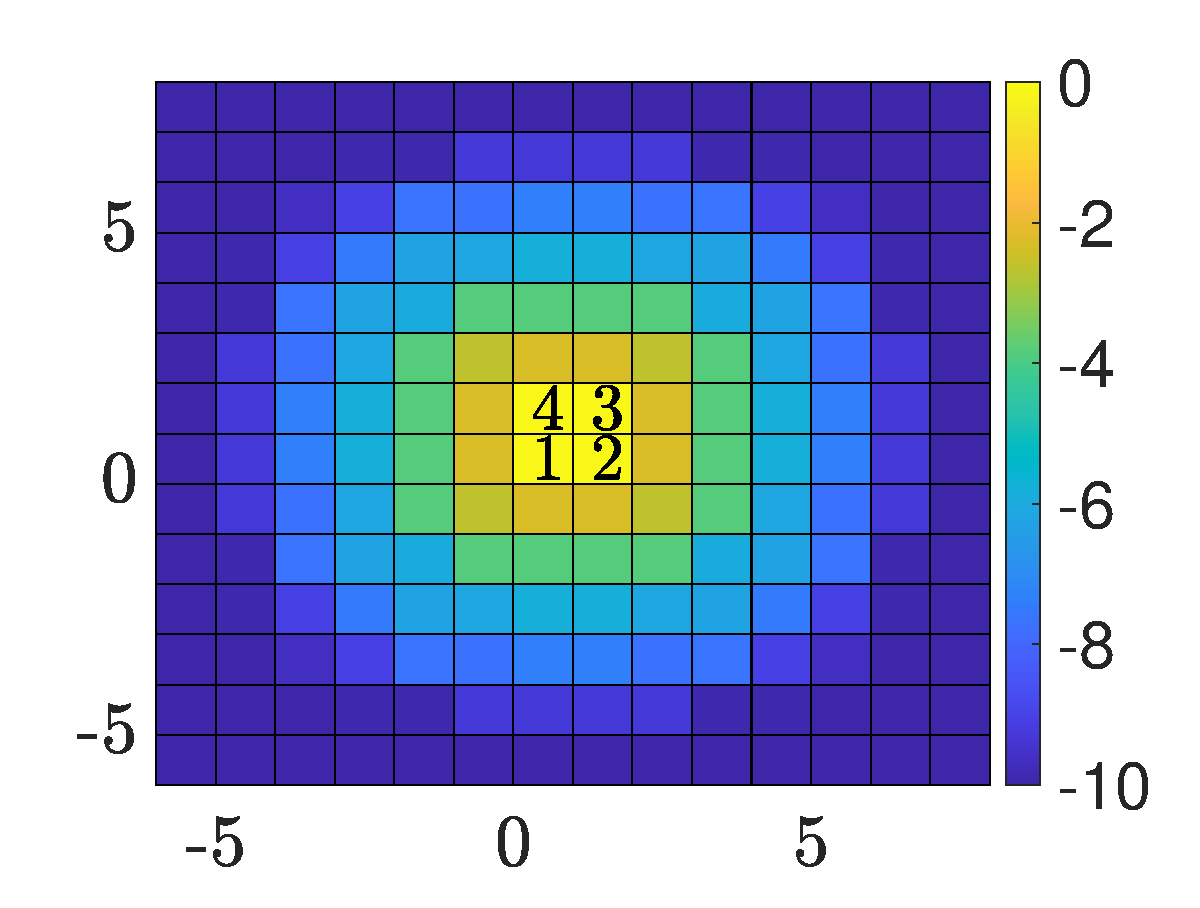
\includegraphics[width=4.5cm]{images/fundc1map.eps}
    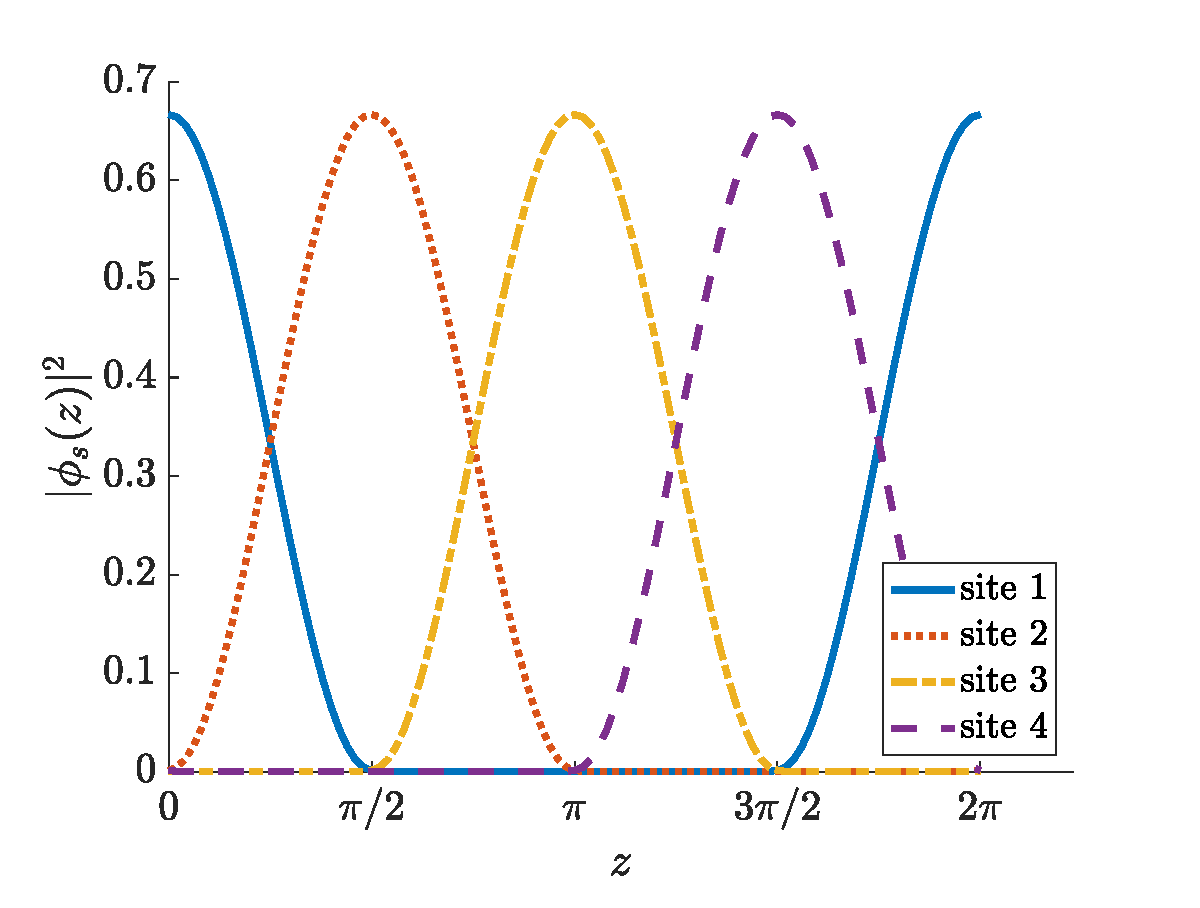
\includegraphics[width=4.5cm]{images/fundc1sol.eps}
    \caption{Cartoon of square lattice with $z$-dependent coupling (left). At any value of $z$, only one of the four coupling functions $J_k(z)$ is nonzero. Log intensity of fundamental breather solution over one period, showing localization to a single unit square in lattice (center). Square intensity of fundamental breather solution on four sites of unit square over one period (right).}
    \label{fig:Rechtsman}
\end{figure} 
Future work involves studying solitons that ``hop'' between adjacent nodes in these optical lattices, and, in particular, the transition between stationary and ``hopping'' solitons.

% \bibliographystyle{amsplain}
% \footnotesize{ \bibliography{researchstatement.bib} }

\end{document}
